\documentclass[11pt]{article}
\usepackage[margin=1in]{geometry}
\usepackage{amsmath,booktabs,graphicx,hyperref,siunitx,enumitem}
\usepackage[T1]{fontenc}
\usepackage{microtype}
\hypersetup{colorlinks=true,linkcolor=blue,citecolor=blue,urlcolor=blue}
\title{Robots at the Door: A Reproducible Discrete-Time Study of Capacity, Arrival Timing, and Queue Pressure}
\author{Robot Invites Working Group}
\date{16 September 2026}
\newcommand{\code}[1]{\texttt{#1}}
\begin{document}
\maketitle

\begin{abstract}
A small party-planning problem provides a compact setting for studying a general systems question: what happens when many agents arrive punctually at a resource with finite capacity? We built a dependency-light Python simulation and p5.js overhead visualization in which robots approach a house and enter through a doorway whose width is measured in robot widths. We compared six interventions: one door, two doors, a wider door, scheduled arrivals, heterogeneous arrival timing, and a larger invite list. Each scenario was run for 20 deterministic seeds under an intentionally synchronized-arrival stress test, with completion time, throughput, admission wait, maximum wait, and peak queue recorded. Two doors doubled modeled admission capacity and halved completion time; widening the door from three to five robot widths improved completion time by 40\%; scheduled arrivals eliminated the queue but extended the arrival window; and increasing the invite list from 30 to 100 robots produced a large persistent queue. These results are claims about this specified toy model, not empirical claims about real robot crowds. We provide source code, machine-readable outputs, figure code, and build instructions.
\end{abstract}

\section{Introduction}
The motivating problem is deliberately ordinary: if every invited robot interprets ``arrive at 9 pm'' literally, the house may receive a large synchronized burst at a doorway that can admit only a few robots at once. The question is not simply how to make robots faster. It is a systems-design question involving capacity, arrival processes, scheduling, spatial layout, and fairness.

This framing has a historical analogue in the development of sensor-mediated interdiction during the Vietnam War. Operation Igloo White used unattended acoustic and seismic sensors, communications relays, computers, and an Infiltration Surveillance Center to collect and interpret information about movement on the Ho Chi Minh Trail \cite{vanstaaveren1993,nalty2005}. The system helped produce predictions and target information that supported air operations. It is important, however, not to describe it anachronistically as a modern machine-learning detector that autonomously called a strike. The historical record describes sensor signals, computer processing, analysts, and a command structure in which strike authority remained outside the sensing system \cite{nalty2005,tilford1991}. Our use of Igloo White is therefore an analogy about sensing, prediction, bottlenecks, and human-machine organization, not a claim that this demonstration recreates its technology or decision process.

The present experiment is a much safer and narrower abstraction: agents are robots attending a party, and the consequence of congestion is waiting rather than harm. It isolates one design principle that queueing theory has studied for more than a century: when demand is concentrated at a resource with finite service capacity, waiting-line characteristics depend jointly on arrival behavior and capacity \cite{kendall1953,gross1998}. The project asks which of the proposed interventions changes which part of that system.

\section{Research Questions}
We investigate four questions:
\begin{enumerate}[leftmargin=*]
\item How strongly does a synchronized arrival surge expose a fixed doorway bottleneck?
\item Does parallel capacity (more doors) outperform increased local capacity (a wider door)?
\item Can arrival scheduling reduce waiting without changing the doorway?
\item What happens when demand grows while capacity remains fixed?
\end{enumerate}

\section{Model}
\subsection{State and geometry}
The Python backend represents each robot $i$ by an identifier, position, status, scheduled arrival time $a_i$, admission time $e_i$, and punctuality multiplier. The default population is $N=30$. The house is represented in overhead two-dimensional coordinates. The baseline door is three robot widths wide and 1.4 robot heights tall. A robot has width and height one in the normalized model.

Time advances in discrete increments of $\Delta t=0.25$ seconds. At each step, all waiting robots satisfying $a_i\leq t$ are eligible. Eligible robots are sorted by identifier and the first $C$ are admitted, where
\begin{equation}
 C = \left\lfloor \frac{w_d}{w_r} \right\rfloor (1+d),
\end{equation}
$w_d$ is door width, $w_r$ is robot width, and $d$ is the number of additional doors. This is a bulk-service approximation: it treats spatial packing as an admission count rather than simulating collision geometry. The service discipline is first-in, first-out.

\subsection{Arrival scenarios}
The experiment harness deliberately sets arrivals to expose differences between interventions. In the synchronized surge, every robot has $a_i=0$. In the invite-timing scenario, arrival times are linearly distributed between 0 and 7 seconds. In the personality scenario, each arrival time is independently sampled from $U(0,3.5)$ using a scenario-specific deterministic seed. The six scenarios are:
\begin{enumerate}[leftmargin=*]
\item one 3-wide door, 30 robots, synchronized surge;
\item two 3-wide doors, 30 robots, synchronized surge;
\item one 5-wide door, 30 robots, synchronized surge;
\item one 3-wide door, 30 scheduled arrivals;
\item one 3-wide door, 30 heterogeneous arrivals;
\item one 3-wide door, 100 robots, synchronized surge.
\end{enumerate}

\subsection{Measurements}
For each run we record:
\begin{align}
 T &= \max_i e_i, && \text{completion time},\\
 Q_{\max} &= \max_t \#\{i:a_i\leq t,\ e_i>t\}, && \text{peak arrived queue},\\
 \bar W &= \frac{1}{N}\sum_i(e_i-a_i), && \text{mean admission wait},\\
 W_{\max} &= \max_i(e_i-a_i), && \text{maximum admission wait},\\
 R &= \frac{60N}{T}, && \text{throughput in robots per minute}.
\end{align}
The backend also emits time-indexed JSONL rows containing inside count, waiting count, not-yet-arrived count, throughput, average wait, maximum wait, door capacity, and utilization.

\section{Reproducible Analysis}
All analysis is implemented in plain Python with no required third-party package for the simulation itself. From the repository root, run:
\begin{verbatim}
python3 run_experiments.py
python3 -m pip install matplotlib numpy
python3 plot_experiments.py
pdflatex manuscript.tex
bibtex manuscript
pdflatex manuscript.tex
pdflatex manuscript.tex
\end{verbatim}
The first command writes \code{experiment-summary.md} and \code{experiment-results.json}; the second reads the JSON and writes \code{figures.pdf}. The LaTeX source and bibliography are \code{manuscript.tex} and \code{references.bib}. The backend is also runnable with \code{python3 backend.py} to inspect the interactive p5.js view.

The experiment uses 20 runs per scenario, with seeds $1000,\ldots,1119$ allocated in contiguous blocks by scenario. The JSON output preserves every individual run, not only means, so later analyses can compute uncertainty intervals or alternative summaries without rerunning the simulation.

\section{Results}
Table~\ref{tab:results} reports means over the 20 runs. In the current model the synchronized scenarios are deterministic after their arrival schedule is imposed, so repeated seeds primarily verify reproducibility; the personality scenario retains run-to-run variation.

\begin{table}[t]
\centering
\caption{Headless experiment results. Values are means over 20 runs.}
\label{tab:results}
\begin{tabular}{lrrrrrrr}
\toprule
Scenario & $N$ & $C$ & $T$ (s) & $R$ (/min) & $\bar W$ (s) & $W_{\max}$ (s) & $Q_{\max}$\\
\midrule
One door & 30 & 3 & 2.5 & 720.0 & 1.4 & 2.5 & 27.0\\
More doors & 30 & 6 & 1.2 & 1440.0 & 0.8 & 1.2 & 24.0\\
Bigger door & 30 & 5 & 1.5 & 1200.0 & 0.9 & 1.5 & 25.0\\
Invite timing & 30 & 3 & 7.0 & 257.1 & 0.1 & 0.2 & 0.0\\
Robot personality & 30 & 3 & 3.6 & 495.9 & 0.2 & 0.7 & 2.6\\
At the limit & 100 & 3 & 8.5 & 705.9 & 4.3 & 8.5 & 97.0\\
\bottomrule
\end{tabular}
\end{table}

\begin{figure}[t]
\centering
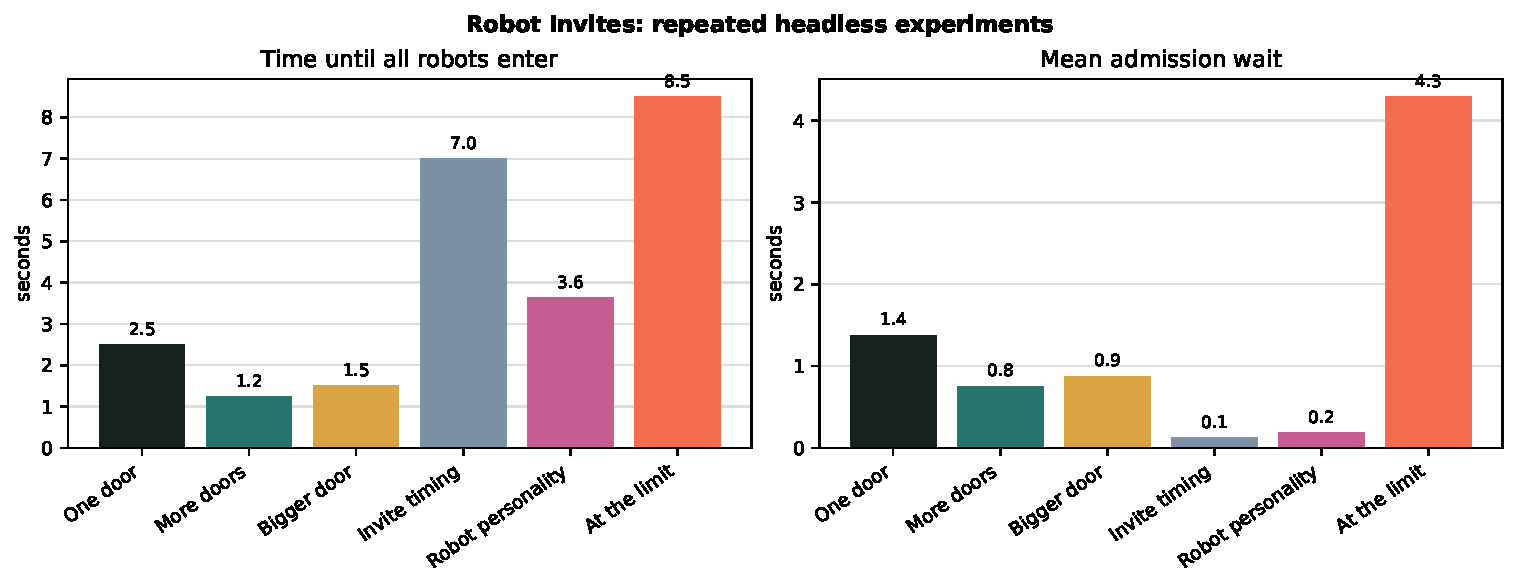
\includegraphics[width=\linewidth]{figures.pdf}
\caption{Results regenerated by \code{plot\_experiments.py} from \code{experiment-results.json}. The left panel measures time to admit the complete population; the right panel measures time from scheduled arrival to admission.}
\label{fig:main}
\end{figure}

Relative to the one-door baseline, two doors reduced completion time to 0.50 times baseline and doubled throughput. The five-wide door reduced completion time to 0.60 times baseline and increased throughput by a factor of 1.67. Scheduled invitations reduced mean wait from 1.4 to 0.1 seconds and reduced peak queue from 27 to zero, but completion time increased because the intervention intentionally spread the arrivals over seven seconds. Personality variation produced an intermediate effect: a 3.6-second completion time, 0.2-second mean wait, and mean peak queue of 2.6 robots. The 100-robot surge required 8.5 seconds, with mean wait 4.3 seconds and peak queue 97 robots.

\section{Discussion}
The results separate two levers that can otherwise be conflated. Structural interventions increase the service rate. Arrival interventions reduce the instantaneous demand rate. Under a synchronized surge, adding a second door is the strongest tested intervention because it doubles $C$ from three to six. Widening the existing opening also helps, but its gain is proportional to the integer packing capacity: changing from three to five widths increases admission capacity by two, not by a factor of two.

Scheduling produces a different tradeoff. It nearly eliminates waiting because the scheduled arrival rate is kept below the doorway's admission rate. This is not a throughput improvement: the total event takes longer because the invitation plan has changed the arrival process. In a real party, this may be desirable if the objective is comfort or social interaction rather than admitting everyone as quickly as possible. A useful extension would therefore treat utility as multi-objective, combining waiting, arrival-window length, fairness, and party occupancy.

The personality intervention is not equivalent to a well-designed schedule. Random variation reduces synchrony but does not guarantee a low queue, and the result depends on its distribution and scale. The present personality scenario is one illustrative distribution, not a general claim that variability is always beneficial. In some regimes, variability could create bursts or unfairly penalize late-arriving robots.

The limit scenario demonstrates the capacity law directly. Holding $C=3$ while increasing $N$ creates a queue whose scale is set by excess demand. This is the same basic reason that queueing analyses track arrival rates, service rates, waiting times, and queue lengths \cite{gross1998,kingman1961}. The model is finite-horizon rather than steady-state, so steady-state formulas should not be applied to these reported numbers without qualification.

The historical analogy also sharpens a systems lesson. Sensor networks and automated or semi-automated command systems do not eliminate uncertainty, interpretation, or governance merely because they add computation. In Igloo White, sensors generated signals, communications moved them, computers organized information, and analysts and command structures interpreted and acted on it. In our demo, the backend similarly separates state generation, metrics, and visualization. That separation makes the experiment inspectable, but it does not make the model authoritative.

\section{Limitations and Future Work}
The model admits robots in FIFO order and does not simulate robot-to-robot collision avoidance, acceleration, turning radius, door-height packing, multiple queues, abandonment, or social preferences. The visual p5.js animation interpolates backend states; it is not part of the measured dynamics. Door capacity is a discrete bulk-service rule, so the unusually high reported robots-per-minute values should be interpreted as rates in normalized simulation time, not as realistic architectural throughput.

Future experiments should add continuous geometry, explicit paths, stochastic service times, queue discipline comparisons, robot size heterogeneity, limited interior capacity, and objective functions for enjoyment or fairness. A stronger validation study would compare the simulator with a continuous-event queue model and would report confidence intervals, not only means. The system could also expose a policy interface so invitation scheduling is optimized against an explicit cost function rather than selected by hand.

\section{Conclusion}
This reproducible demonstration turns a playful party problem into a transparent study of finite capacity and synchronized demand. The principal result is conditional but clear: if all robots arrive together, structural capacity dominates; if the goal is low waiting rather than rapid completion, arrival scheduling is powerful; and if the population grows without capacity growth, the bottleneck becomes unavoidable. The code and machine-readable outputs make those claims easy to inspect, challenge, and extend.

\bibliographystyle{plain}
\bibliography{references}
\end{document}
